\documentclass[border=8pt]{standalone}
\usepackage{pgfplots}
\pgfplotsset{compat=1.18}
\begin{document}
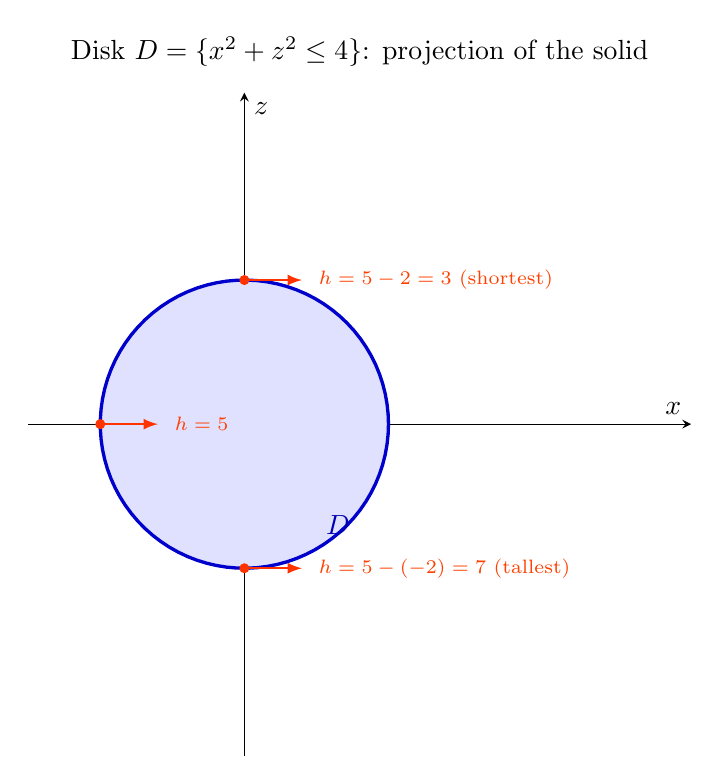
\begin{tikzpicture}
\begin{axis}[
    width=10cm, height=10cm, axis equal,
    xmin=-3.0, xmax=6.2, ymin=-3.2, ymax=3.2,
    axis lines=middle, xtick=\empty, ytick=\empty,
    xlabel=$x$, ylabel=$z$,
    title={Disk $D=\{x^2+z^2\le 4\}$: projection of the solid}]
    \addplot[blue!12, fill, draw=none, domain=0:360, samples=90] ({2*cos(x)}, {2*sin(x)});
    \addplot[very thick, blue!80!black, domain=0:360, samples=90] ({2*cos(x)}, {2*sin(x)});
    \addplot[only marks, mark=*, mark size=1.6pt, red!60!orange] coordinates {(0,2) (-2,0) (0,-2)};
    \draw[-latex, thick, red!60!orange] (axis cs:0,2)    -- (axis cs:0.8,2);
    \draw[-latex, thick, red!60!orange] (axis cs:-2,0)   -- (axis cs:-1.2,0);
    \draw[-latex, thick, red!60!orange] (axis cs:0,-2)   -- (axis cs:0.8,-2);
    \node[anchor=west, font=\scriptsize, text=red!50!orange] at (axis cs:0.9,2)  {$h=5-2=3$ (shortest)};
    \node[anchor=west, font=\scriptsize, text=red!50!orange] at (axis cs:-1.1,0) {$h=5$};
    \node[anchor=west, font=\scriptsize, text=red!50!orange] at (axis cs:0.9,-2) {$h=5-(-2)=7$ (tallest)};
    \node[blue!70!black] at (axis cs:1.3,-1.4) {$D$};
\end{axis}
\end{tikzpicture}
\end{document}
